\documentclass[12pt]{article}
\everymath{\displaystyle}
\usepackage{unicode-math}
\usepackage{pgfplots}
\pgfplotsset{compat=1.18}
\usepackage{amsmath}


\usepackage[margin=1in]{geometry}
\usepackage{tcolorbox}
\usepackage{graphicx}
\usepackage{tikz}
\usepackage{amssymb}
\usepackage{enumitem}
\usepackage{titlesec}
\usepackage{fancyhdr}
\usepackage{pifont}
\usepackage{xcolor}
\newcounter{questionnum}
\setcounter{questionnum}{0}
\usepackage{eso-pic} % for page background



\usepackage{booktabs}
\usepackage{tabularx}
\usepackage{titlesec}
\usepackage{helvet}


\titleformat{\section}{\Large\bfseries}{\thesection}{1em}{}
\titleformat{\subsection}{\large\bfseries}{\thesubsection}{1em}{}
\titleformat{\subsubsection}{\normalsize\bfseries}{\thesubsubsection}{1em}

% --------- 主题颜色设置 ---------
\definecolor{novelblue}{RGB}{70,60,150}
\definecolor{headerbg}{RGB}{240,240,255}

\pagestyle{fancy}
\fancyhf{}
\renewcommand{\headrulewidth}{0.4pt}
\renewcommand{\headrule}{\hbox to\headwidth{\color{novelblue}\leaders\hrule height 0.4pt\hfill}}

% --------- 页眉背景色条 ---------
\newcommand{\headbackground}{
  \AddToShipoutPictureBG*{
    \begin{tikzpicture}[remember picture, overlay]
      \fill[blue!5!purple!10] (current page.north west) rectangle ([yshift=-60pt]current page.north east);
    \end{tikzpicture}
  }
}

% --------- 页眉设置 ---------
\pagestyle{fancy}
\fancyhf{}
\renewcommand{\headrulewidth}{0pt}
\fancyhead[L]{\color{novelblue}\textbf{\textbf{Novel Prep} }}
\fancyhead[C]{\color{novelblue}\textbf {SAT Preparation}}
\fancyhead[R]{\color{novelblue}\textbf{Jack Zeng}}


\newtcolorbox{SATCard}[1][]{%
  enhanced,
  colback=white,
  colframe=novelblue,
  coltitle=white,
  boxrule=0.6pt,
  arc=4pt,
  boxsep=5pt,
  left=8pt, right=8pt, top=10pt, bottom=10pt,
  sharp corners=south,
  drop shadow south east,
  #1
}

% --------- 顶部 Mark for Review 栏 ---------
\newcommand{\markforreview}{
  \stepcounter{questionnum} % 自动递增题号
  \begin{tikzpicture}[scale=1.1]
    % 黑色题号
    \fill[black] (0,0) rectangle (0.8,0.6);
    \node[white, font=\bfseries\large] at (0.4,0.3) {\thequestionnum};

    % 灰底主栏
    \fill[gray!10] (0.8,0) rectangle (14.5,0.6);

    % Mark for Review
    \node[anchor=west, font=\small] at (1.2,0.3) {\ding{72} \hspace{2pt}Mark for Review};

    % ABC 按钮区域
    \draw[thick, rounded corners=3pt] (13.5,0.12) rectangle (14.5,0.48);
    \node[font=\bfseries\normalsize] at (14.0,0.3) {ABC};
  \end{tikzpicture}


  \newcommand{\choiceboxcircled}[2]{%
  \begin{tcolorbox}[
    colback=white,
    colframe=black,
    boxrule=0.5pt,
    rounded corners=6pt,
    left=6pt, right=6pt, top=6pt, bottom=6pt,
    width=\linewidth
  ]
    \textbf{\large\textcircled{\textbf{#1}}} \ #2
  \end{tcolorbox}
}
}

% --------- 选项框样式 ---------
\newcommand{\choicebox}[2]{%
  \begin{tcolorbox}[
    colback=white, 
    colframe=novelblue,
    boxrule=0.5pt, 
    rounded corners=4pt, 
    left=6pt, right=6pt, top=6pt, bottom=6pt,
    width=\linewidth
  ]
  \textbf{#1.} \ #2
  \end{tcolorbox}
}


\begin{document}
\section*{SAT Module II Test}
\noindent\markforreview
\vspace{1em}

For the function
\[
f(x) = a\sqrt{x-b} + 12\sqrt{x-b},
\]
$a$ and $b$ are constants, and $f(4)=0$. If $f(5) > 0$, which of the following could be a value for $a+b$?

\vspace{0.75em}

\choicebox{A}{-20}  
\choicebox{B}{-12}  
\choicebox{C}{-8}  
\choicebox{D}{-4}

\vspace{2em}

\noindent\markforreview
\vspace{1em}

\[
\frac{16}{a}=\frac{16}{b}+\frac{16}{c}
\]

Which of the following expresses $a$ in terms of $b$ and $c$?

\vspace{0.75em}

\choicebox{A}{$a=\dfrac{b+c}{bc}$}  
\choicebox{B}{$a=\dfrac{bc}{b+c}$}  
\choicebox{C}{$a=bc(b+c)$}  
\choicebox{D}{$a=16bc(b+c)$}

\newpage


\vspace{2em}


\noindent\markforreview
\vspace{1em}

\[
\frac{ax^{3}+bx^{2}+cx+d}{(x^{2}-9)(x+2)}
\;=\;
\frac{5}{x+3}+\frac{6x}{x-3}
\]

What is the value of $a+b+c$?

\vspace{5em}

\noindent\markforreview
\vspace{1em}

There are two lawn mowing companies. Company A charges a flat fee of \$80 for the first hour, then an hourly rate of \$60 for each additional hour.  
Company B charges no flat fee, but an hourly rate of \$75 per hour.  
After how many \textit{minutes} will company B's total cost exceed company A's?

\vspace{5em}
\noindent\markforreview


\[
\frac{5}{6}x + ay = b
\]
\[
\frac{11}{10}x + cy = 2d
\]

If the system of equations above has infinite solutions, what must be the value of $\dfrac{b}{d}$?

\vspace{5em}
\noindent\markforreview
\vspace{1em}

$a$ is $540\%$ more than $b$ and $b$ is $0.02\%$ of $c$
If $a$ is $k\%$ of $c$, then what must $k$ equal?

\newpage

\noindent\markforreview
\vspace{1em}

\[
f(t)=a\cdot 2^{\frac{2t}{11}}
\]

The given function $f(t)$ models the amount of money in an investment account $t$ years after the account is opened, where $a$ is a constant.  
How many months will it take for the initial investment to increase by $700\%$?

% ----------------------------------------------------

\vspace{2em}
\noindent\markforreview
\vspace{1em}

\[
f(x)=k^{3}(k^{x})+b
\]

The function $f$ is defined by the equation above for $x\ge 0$.  
$k$ and $b$ are positive constants and $k<1$. Which of the following must be true?

\begin{itemize}
\item[I.] The maximum value of the function is displayed as a constant or coefficient of the function.
\item[II.] $f(1)=f(0)\cdot k$
\item[III.] $f(a)<b$ for some $a>0$
\end{itemize}

\vspace{0.75em}

\choicebox{A}{I only}  
\choicebox{B}{II and III only}  
\choicebox{C}{I and III only}  
\choicebox{D}{Neither I, II, nor III}

\vspace{3em}

\noindent\markforreview
\vspace{1em}

\[
15x^{18} + kx^{9} + 24
\]

The expression above has factors $ax^{9}+b$ and $cx^{9}+d$, where $a$, $b$, $c$, and $d$ are all integer constants.  
What is the maximum value of $k$?


\newpage

\noindent\markforreview
\vspace{1em}

\[
(hx+k)(qx+z) = ax^{2} + bx + 35
\]

For the expression above, $h, k, q,$ and $z$ are all integer constants.  
Which of the following must be an integer?

\begin{itemize}
\item[I.] $\dfrac{35}{k}$
\item[II.] $b$
\item[III.] $-\dfrac{a}{q}$
\end{itemize}

\vspace{0.75em}

\choicebox{A}{I and II only}  
\choicebox{B}{II and III only}  
\choicebox{C}{I and III only}  
\choicebox{D}{I, II, and III}

\newpage

\noindent\markforreview
\vspace{1em}

\[
f(x)=-3x^{2}+bx+c
\]

In the given quadratic function, $b$ and $c$ are constants. The graph of $y=f(x)$ in the xy-plane is a parabola that has a vertex at the point $(h,k)$, where $h$ and $k$ are constants. If $f(-4)=f(8)$, and the quadratic function has x-intercepts at $(r,0)$ and $(s,0)$, which of the following must be true?

\begin{itemize}
\item[I.] $r+s=4$
\item[II.] $b<0$
\item[III.] $c<k$
\end{itemize}

\vspace{0.75em}

\choicebox{A}{I and II only}  
\choicebox{B}{II and III only}  
\choicebox{C}{I and III only}  
\choicebox{D}{I, II, and III}  

\vspace{4em}

\noindent\markforreview
\vspace{1em}

A quadratic function models a rock's height, in feet, above the ground in terms of the time, in seconds, after it is thrown. 
The rock was thrown from an initial height of $c$ feet above the ground and reached a maximum height of 200 feet above the ground 3 seconds after it was thrown. 
Then it hit the ground 8 seconds after being thrown. 
At what initial height $c$ was the rock thrown?


\newpage

\noindent\markforreview
\vspace{1em}

\[
2rx^{2}-5sx+8r=0
\]

If the quadratic equation above has one real solution and $rs=160$, what is $\lvert r+s\rvert$?



\vspace{2em}

\noindent\markforreview
\vspace{1em}

\[
f(x)=-(x+a)^{2}(x-b)(x-c)
\]

For the polynomial function above, $a$, $b$, and $c$ are positive constants.  
Let $b<k<c$ for some constant $k$. Which of the following must be true?

\begin{itemize}
\item[I.] $k>0$
\item[II.] $f(k)>0$
\item[III.] $f(0)>0$
\end{itemize}

\vspace{0.75em}

\choicebox{A}{I and II only}  
\choicebox{B}{II and III only}  
\choicebox{C}{I and III only}  
\choicebox{D}{I, II, and III}


\newpage
\noindent\markforreview
\vspace{1em}

3 consecutive even integers are ordered from smallest to largest. 
5 times the first integer is at least 9 more than the sum of the second and third integers. 
What is the minimum possible value for the second integer?



\vspace{5em}
\noindent\markforreview
\vspace{1em}

If a car accelerates at $108$ kilometers per hour squared, what is its acceleration in meters per minute squared? 
\;(1 kilometer $= 1000$ meters)


\vspace{3em}


\noindent\markforreview
\vspace{1em}

In triangle $\triangle ABC$, the measure of $\angle B$ is $90^\circ$, $\overline{AB}$ is a leg with a length of $12$, and point $D$ lies on segment $\overline{AC},$ and finally connect $BD$.
Which of the following must be true?

\begin{itemize}
\item[I.] $\overline{BC}=12\,\tan(\angle CAB)$
\item[II.] $\cos(\angle ABD)-\sin(\angle DBC)=0$
\item[III.] $\angle ABD=\angle BDC$
\end{itemize}

\vspace{0.75em}

\choicebox{A}{I and II only}  
\choicebox{B}{II and III only}  
\choicebox{C}{I and III only}  
\choicebox{D}{I, II, and III}

\vspace{2em}

\noindent\markforreview
\vspace{1em}

In triangle $\triangle ABC$, the measure of $\angle B$ is $90^\circ$, and $\overline{BD}$ is an altitude of the triangle. 
The length of $\overline{BC}$ is $10$ and $\angle ABD=60^\circ$. 
What is the length of $\overline{AD}$?


\newpage
\noindent\markforreview
\vspace{1em}
\begin{center}
    


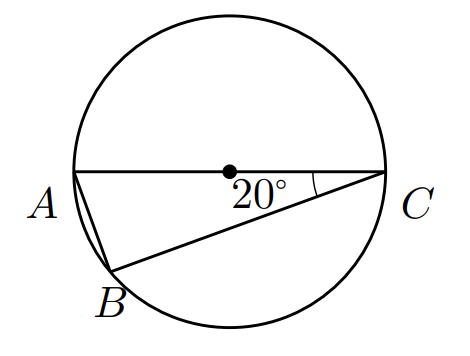
\includegraphics[width=0.3\linewidth]{f16.png}
\end{center}

In the circle above, the angle at point $C$ measures $20^\circ$ and $\overline{AC}$ is a diameter (as shown).  
If the circumference of the circle is $90$ inches, what is the length of arc $BC$?

\vspace{7em}

\noindent\markforreview
\vspace{1em}

In the xy-plane, the graph of $x^{2}+6x+y^{2}+2y=15$ is a circle. 
Line $k$ has a slope of $\tfrac{3}{4}$ and is tangent to this circle at the point $(a,b)$, where $b$ is negative. 
What is the value of $b$?






\vspace{7em}


\noindent\markforreview
\vspace{1em}

Rectangular prism A and rectangular prism B are similar. 
The height of rectangular prism A is $4$ inches and the height of rectangular prism B is $10$ inches. 
If the volume of prism A is $200$ cubic inches, then what is the volume of prism B?


\vspace{7em}


\noindent\markforreview
\vspace{1em}

Consider a square right pyramid with a volume of $400$ cubic inches and a slant height of $13$ inches. 
The pyramid's length, width, and height (in inches) are all integers. 
What is the surface area of the pyramid in cubic inches?

\newpage

\noindent\markforreview
\vspace{1em}

Data set A consists of $4$ integers greater than or equal to $10$ but less than or equal to $20$. 
Data set B consists of the same four integers and adds one more integer, which must also be between $10$ and $20$. 
What is the largest possible difference between the mean of data set A and the mean of data set B?


\vspace{4em}



\noindent\markforreview
\vspace{1em}

\begin{center}
\begin{tabular}{|c|c|}
\hline
\textbf{Data} & \textbf{Frequency}\\
\hline
1 & 2\\
2 & 5\\
3 & 6\\
4 & 5\\
5 & 2\\
\hline
\end{tabular}
\end{center}

The frequency table above summarizes data set A. 
Data set B is created by multiplying all of the values in data set A by $2$. 
Which of the following must be true?

\begin{itemize}
\item[I.] The difference between the mean and median of data set B is $0$.
\item[II.] The standard deviation of data set B is equal to the standard deviation of data set A.
\item[III.] The range of data set B is double the range of data set A.
\end{itemize}

\vspace{0.75em}

\choicebox{A}{I and II only}  
\choicebox{B}{II and III only}  
\choicebox{C}{I and III only}  
\choicebox{D}{I, II, and III}
\newpage
\noindent\markforreview
\vspace{1em}

A sample of students was selected at random from all 11th graders in at a school. 
Based on the sample, it is estimated that the proportion of 11th graders in at least one AP class is $60\%$ with a margin of error of $5\%$. 
Which of the following conclusions are appropriate?

\begin{itemize}
\item[I.] It is not possible for just $40\%$ of the 11th graders in the school to be in at least one AP class.
\item[II.] It is plausible that the proportion of \emph{all students at the school} in at least one AP class is between $45\%$ and $55\%$.
\item[III.] If the sample size is increased, the margin of error will drop below $5\%$.
\end{itemize}

\vspace{0.75em}

\choicebox{A}{I and II only}  
\choicebox{B}{II and III only}  
\choicebox{C}{III only}  
\choicebox{D}{I, II, and III}































\end{document}